\documentclass[pdflatex,compress,mathserif]{beamer}

%\usetheme[dark,framenumber,totalframenumber]{ElektroITK}
\usetheme[darktitle,framenumber,totalframenumber]{ElektroITK}

\usepackage[utf8]{inputenc}
\usepackage[T1]{fontenc}
\usepackage{lmodern}
\usepackage[bahasai]{babel}
\usepackage{amsmath}
\usepackage{amsfonts}
\usepackage{amssymb}
\usepackage{graphicx}
\usepackage{multicol}

\newcommand*{\Scale}[2][4]{\scalebox{#1}{$#2$}}%

\setbeamertemplate{caption}[numbered]
\setbeamertemplate{section in toc}[sections numbered]

\title{Sinyal dan Sistem}
\subtitle{Sinyal dan Sistem}

\author{Tim Dosen Pengampu}

\begin{document}

\maketitle

\section{Sinyal Waktu Kontinyu dan Sinyal Waktu Diskrit}

\begin{frame}
	\frametitle{Sinyal}
	\begin{center}
		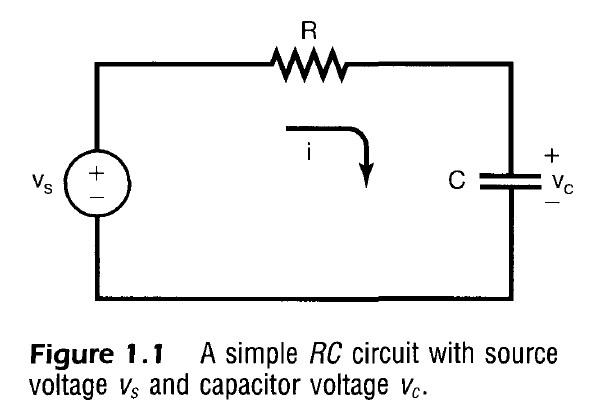
\includegraphics[width=0.7\linewidth]{img/img01}
	\end{center}
\end{frame}

\begin{frame}{Sinyal}
	\begin{center}
		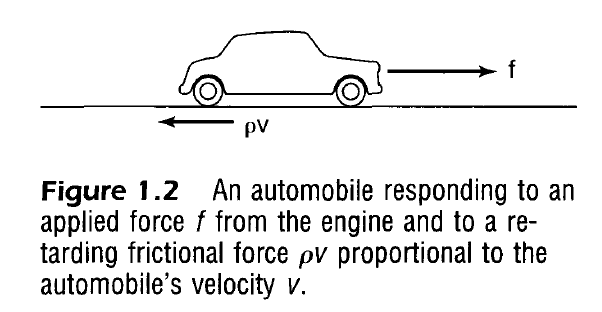
\includegraphics[width=0.7\linewidth]{img/img02}
	\end{center}
\end{frame}

\begin{frame}{Sinyal}
	\begin{center}
		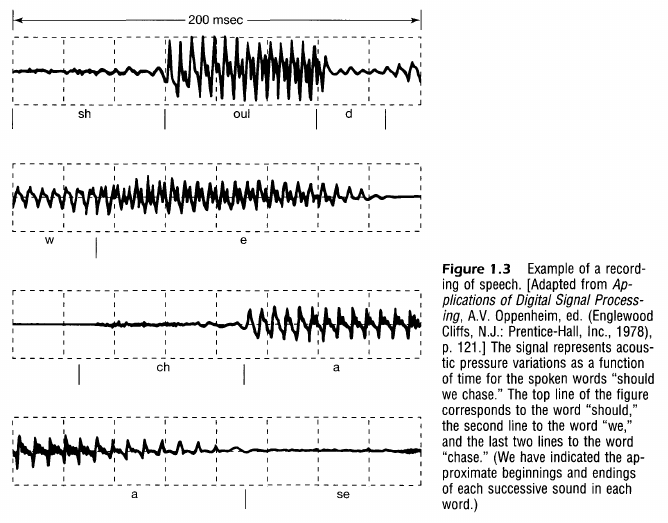
\includegraphics[width=0.7\linewidth]{img/img03}
	\end{center}
\end{frame}

\begin{frame}{Sinyal}
	\begin{center}
		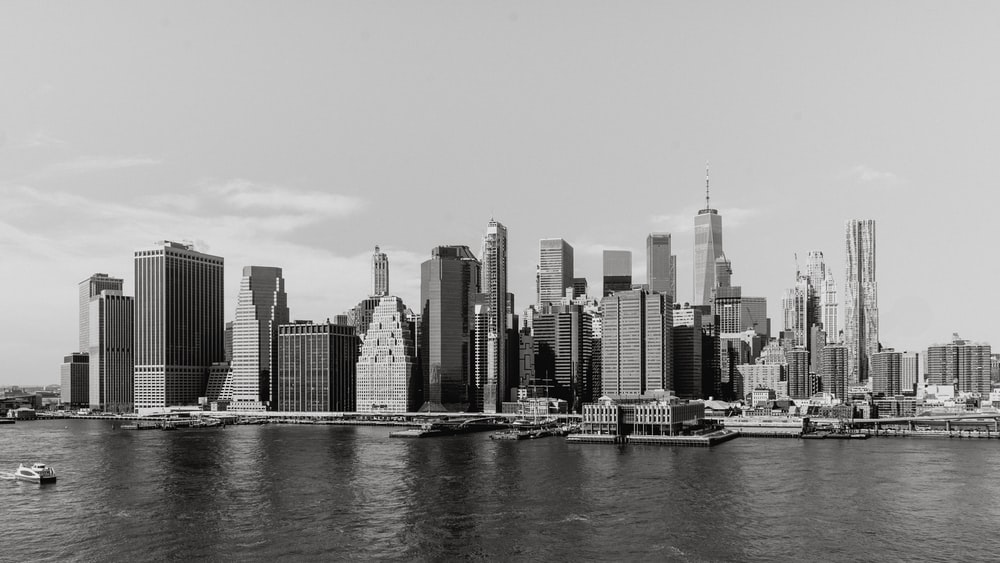
\includegraphics[width=0.7\linewidth]{img/img04}
	\end{center}
\end{frame}

\begin{frame}{Sinyal}
	\begin{center}
		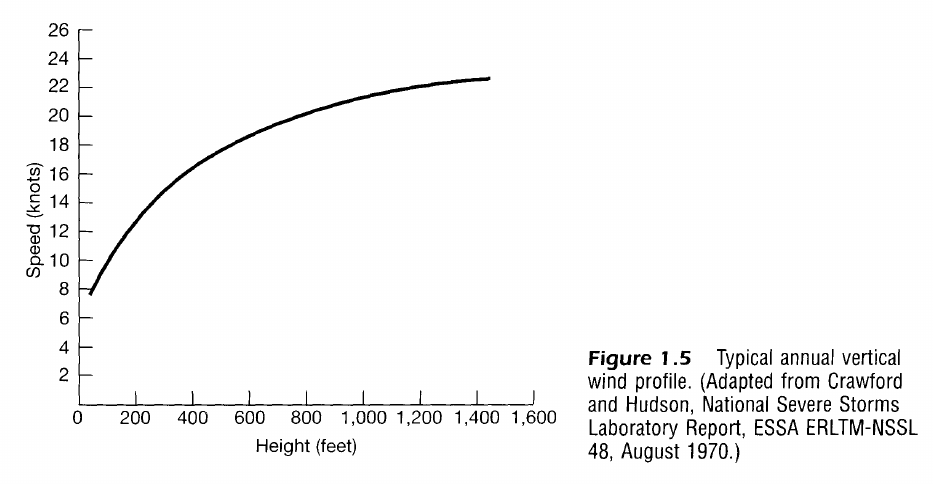
\includegraphics[width=0.7\linewidth]{img/img05}
	\end{center}
\end{frame}

\begin{frame}{Sinyal}
	\begin{enumerate}
		\item Sinyal waktu kontinyu
		\item Sinyal waktu diskrit
	\end{enumerate}
\end{frame}

\begin{frame}{Sinyal}
	\begin{center}
		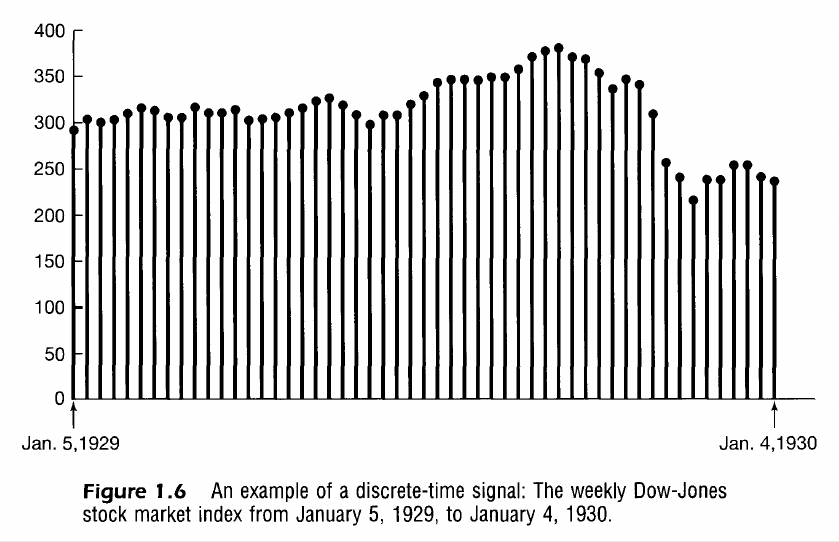
\includegraphics[width=0.7\linewidth]{img/img06}
	\end{center}
\end{frame}

\begin{frame}{Sinyal}
	\begin{enumerate}
		\item Notasi sinyal waktu kontinyu x(t)
		\item Notasi sinyal waktu diskrit x[n]
	\end{enumerate}
\end{frame}

\begin{frame}{Sinyal}
	\begin{center}
		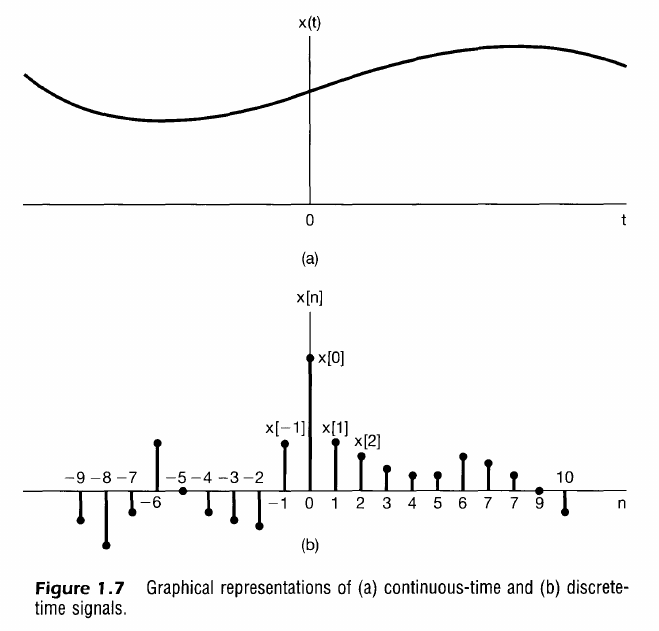
\includegraphics[width=0.7\linewidth]{img/img07}
	\end{center}
\end{frame}

\begin{frame}
	\frametitle{Daya dan Energi Sinyal}
	\begin{multicols}{2}
		\begin{center}
			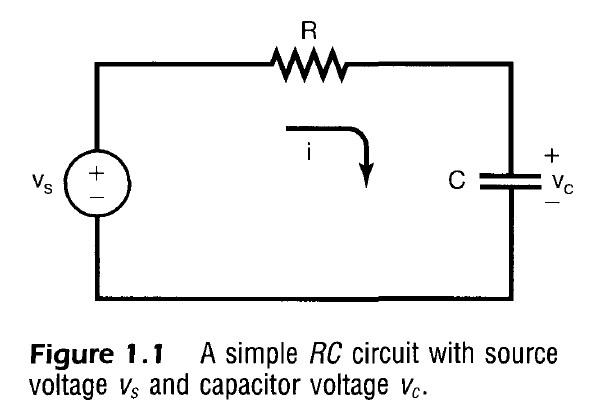
\includegraphics[width=\linewidth]{img/img01}
		\end{center}
		\columnbreak
		Daya:\\
		\begin{center}
			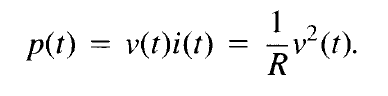
\includegraphics[width=0.7\linewidth]{img/img08}
		\end{center}
		Energi total:\\
		\begin{center}
			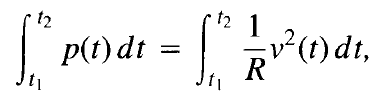
\includegraphics[width=0.7\linewidth]{img/img09}
		\end{center}
		Daya rata-rata:\\
		\begin{center}
			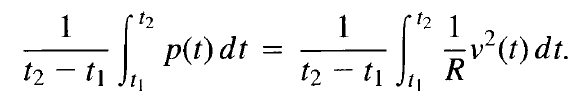
\includegraphics[width=\linewidth]{img/img10}
		\end{center}
	\end{multicols}
\end{frame}

\begin{frame}{Daya dan Energi Sinyal}
	\begin{multicols}{2}
		\begin{center}
			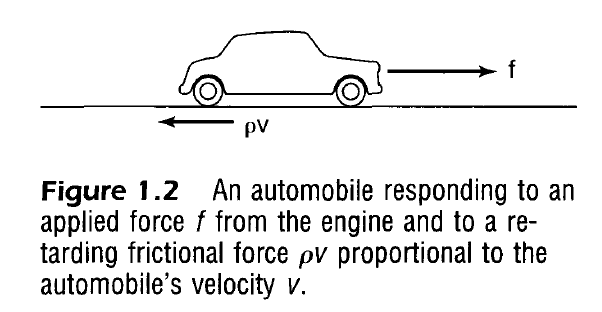
\includegraphics[width=\linewidth]{img/img02}
		\end{center}
		\columnbreak
		Daya:\\
		\begin{center}
			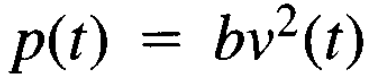
\includegraphics[width=0.5\linewidth]{img/img11}
		\end{center}
		Energi total: ? \\
		Daya rata-rata: ?\\
	\end{multicols}
\end{frame}

\begin{frame}{Daya dan Energi Sinyal}
	\begin{itemize}
		\item Energi total dalam interval $ t_1 \leq t \leq t_2 $ dalam sinyal waktu kontinyu $ x(t) $
		\begin{center}
			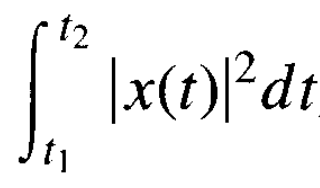
\includegraphics[width=0.2\linewidth]{img/img12}
		\end{center}
		$ |x(t)| $ adalah magnitude dari $ x $
		
		\item Energi total dalam interval $ n_1 \leq n \leq n_2 $ dalam sinyal waktu diskrit $ x[n] $
		\begin{center}
			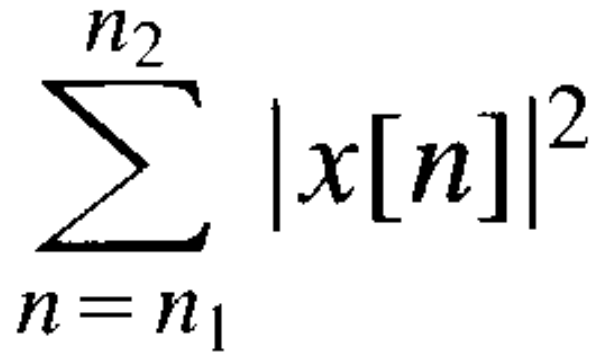
\includegraphics[width=0.2\linewidth]{img/img13}
		\end{center}
		$ |x(n)| $ adalah magnitude dari $ x $
	\end{itemize}
\end{frame}

\begin{frame}{Daya dan Energi Sinyal}
	\begin{itemize}
		\item Energi total dalam interval $ -\infty \leq t \leq \infty $ dalam sinyal waktu kontinyu $ x(t) $
		\begin{center}
			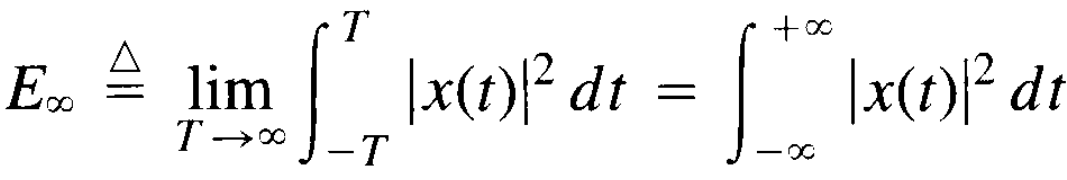
\includegraphics[width=0.5\linewidth]{img/img14}
		\end{center}
		
		\item Energi total dalam interval $ -\infty \leq n \leq \infty $ dalam sinyal waktu diskrit $ x[n] $
		\begin{center}
			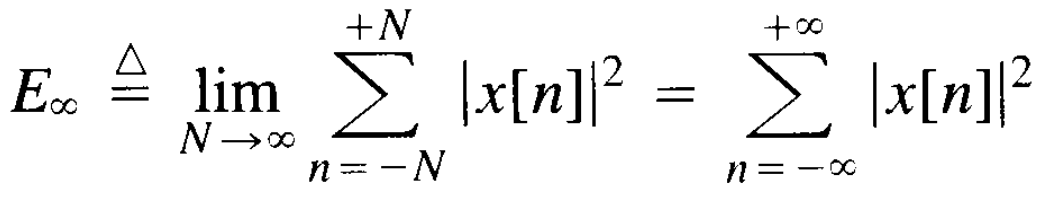
\includegraphics[width=0.5\linewidth]{img/img15}
		\end{center}
		
		\item Kedua persamaan di atas bisa saja tidak konvergen.
		\item Jika $ x(t) $ dan $ x[n] $ sama dengan konstanta bukan nol di semua $ t $, maka sinyal tersebut memiliki energi yang tak hingga. Sedangkan sinyal dengan $ E_{\infty} < \infty $ memiliki energi berhingga.
	\end{itemize}
\end{frame}

\begin{frame}{Daya dan Energi Sinyal}
	\begin{itemize}
		\item Daya rata-rata dalam interval $ -\infty \leq t \leq \infty $ dalam sinyal waktu kontinyu $ x(t) $
		dan sinyal waktu diskrit $ x[n] $
		\begin{center}
			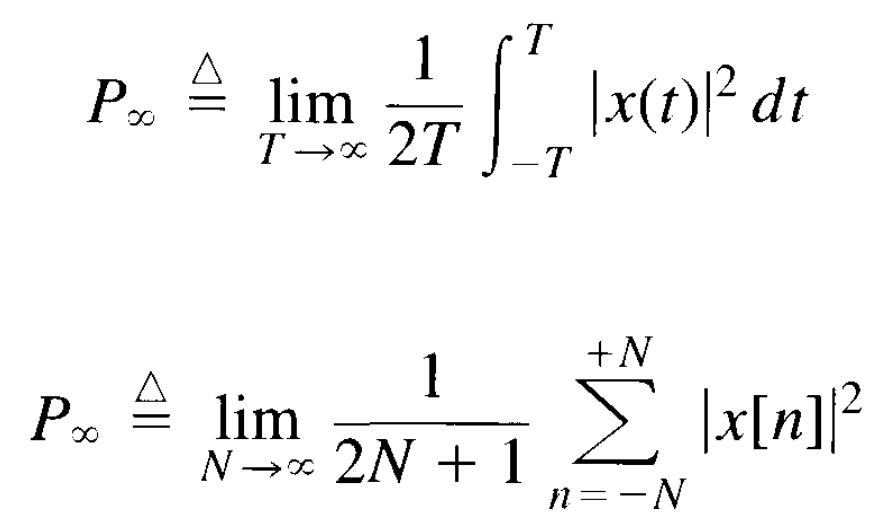
\includegraphics[width=0.5\linewidth]{img/img16}
		\end{center}
		
	\end{itemize}
\end{frame}

\begin{frame}{Daya dan Energi Sinyal}
	Berdasarkan persamaan-persamaan tadi, dapat disimpulkan bahwa terdapat 3 jenis sinyal:
	\begin{enumerate}
		\item Sinyal dengan total energi berhingga $ E_{\infty} < \infty $. Sinyal ini memiliki daya rata-rata yang bernilai nol
		\begin{center}
			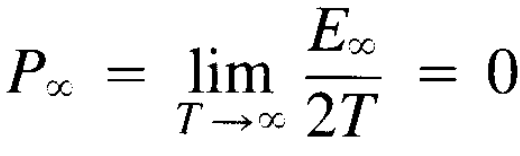
\includegraphics[width=0.3\linewidth]{img/img17}
		\end{center}
		Contoh sinyal dengan total energi berhingga yang bernilai 1 untuk $ 0 \leq t \leq 1 $ dan bernilai 0 di lainnya. Pada kasus ini, $ E_{\infty} = 1 $ dan $ P_{\infty} = 0 $
		\item Sinyal dengan daya rata-rata berhingga. Jika $ P_{\infty} > 0 $, maka $ E_{\infty} = \infty $.
		\item Sinyal yang baik $ P_{\infty} $ maupun $ E_{\infty} $ nya tidak berhingga.
	\end{enumerate}
\end{frame}

\section{Transformasi Variabel Bebas}

\begin{frame}
	\frametitle{Transformasi variabel bebas}
	\begin{itemize}
		\item Time-shift
		\begin{center}
			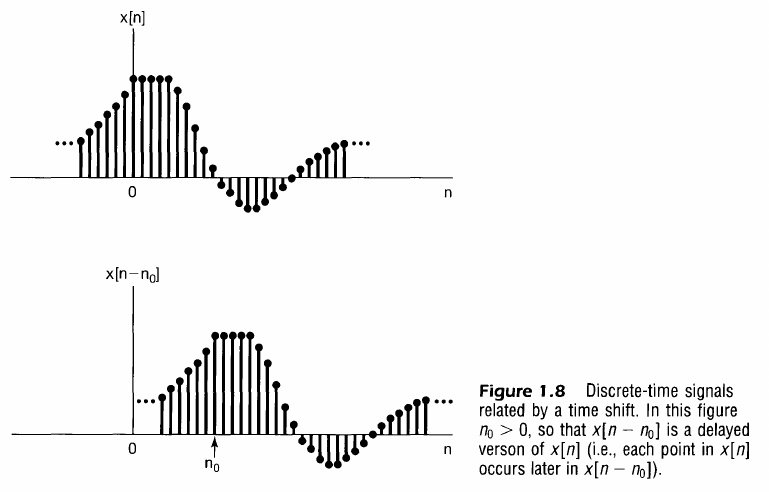
\includegraphics[width=0.8\linewidth]{img/img18}
		\end{center}
	\end{itemize}
\end{frame}

\begin{frame}{Transformasi variabel bebas}
	\begin{itemize}
		\item Time-shift
		\begin{center}
			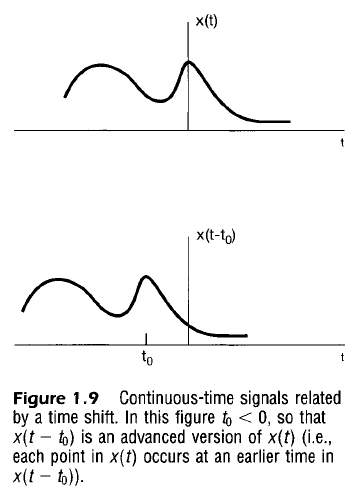
\includegraphics[width=0.4\linewidth]{img/img19}
		\end{center}
	\end{itemize}
\end{frame}

\begin{frame}{Transformasi variabel bebas}
	\begin{itemize}
		\item Time-reversal
		\begin{center}
			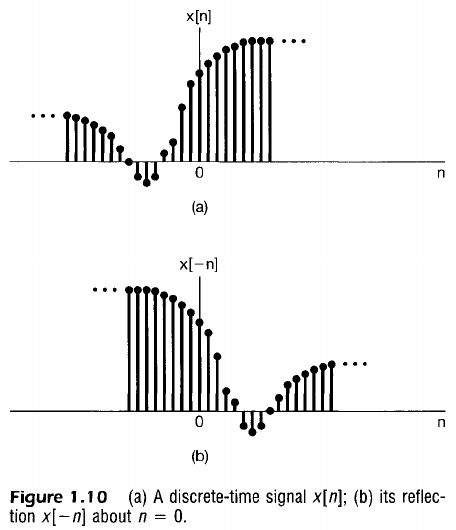
\includegraphics[width=0.4\linewidth]{img/img20}
		\end{center}
	\end{itemize}
\end{frame}

\begin{frame}{Transformasi variabel bebas}
	\begin{itemize}
		\item Time-reversal
		\begin{center}
			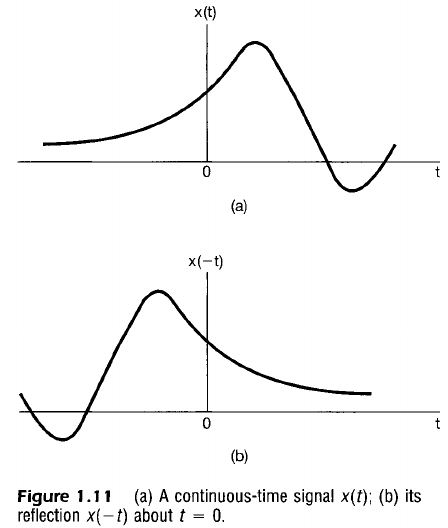
\includegraphics[width=0.5\linewidth]{img/img21}
		\end{center}
	\end{itemize}
\end{frame}

\begin{frame}{Transformasi variabel bebas}
	\begin{itemize}
		\item Scaling
		\begin{center}
			
\includegraphics[width=0.4\linewidth]{img/img22}
		\end{center}
	\end{itemize}
\end{frame}

\begin{frame}
	\frametitle{Contoh transformasi variabel bebas}
	\begin{itemize}
		\item Scaling
		\begin{center}
			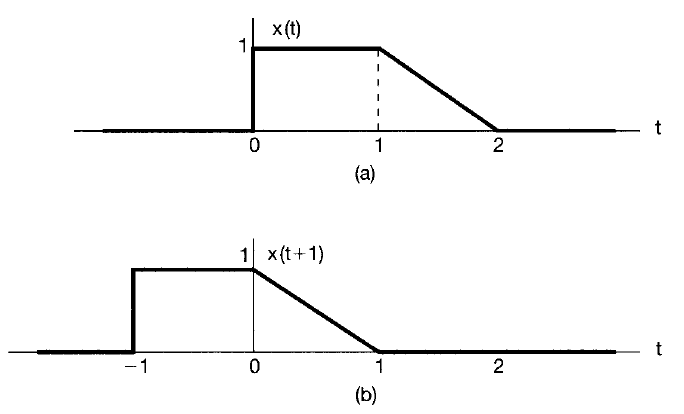
\includegraphics[width=0.7\linewidth]{img/img23}
		\end{center}
	\end{itemize}
\end{frame}

\begin{frame}{Contoh transformasi variabel bebas}
	\begin{itemize}
		\item Scaling
		\begin{center}
			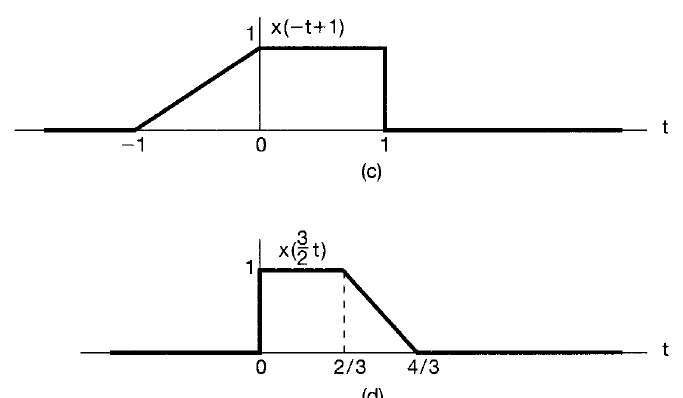
\includegraphics[width=0.7\linewidth]{img/img24}
		\end{center}
	\end{itemize}
\end{frame}

\begin{frame}{Contoh transformasi variabel bebas}
	\begin{itemize}
		\item Scaling
		\begin{center}
			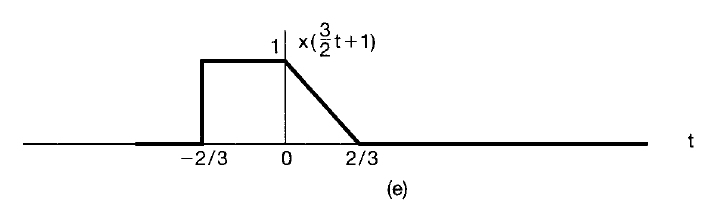
\includegraphics[width=0.7\linewidth]{img/img25}
		\end{center}
	\end{itemize}
\end{frame}

\section{Sinyal Periodik}

\begin{frame}
	\frametitle{Sinyal Periodik}
	\begin{itemize}
		\item Sinyal periodik waktu kontinyu $ x(t) = x(t + T) $
		\begin{center}
			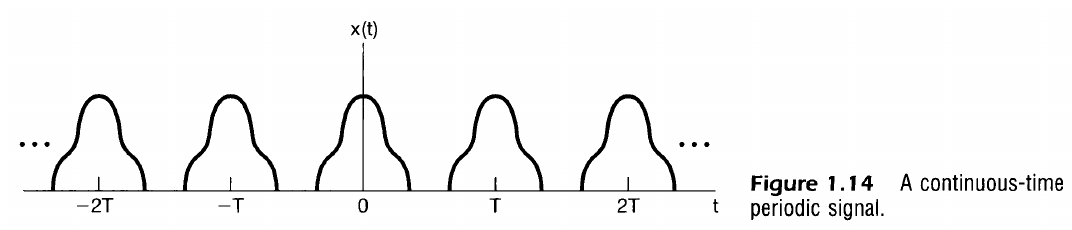
\includegraphics[width=\linewidth]{img/img26}
		\end{center}
		\item Sifatnya tidak berubah dengan time-shift sebesar $ T $
		\item Jika $ x(t) $ adalah periodik dengan periode $ T $, maka $ x(t) = x(t + mT) $
		\item $ T_0 $ adalah periode dasar, yaitu nilai positif terkecil dari T
		\item Sinyal $ x(t) $ yang tidak periodik disebut sinyal aperiodik
	\end{itemize}
\end{frame}

\begin{frame}{Sinyal Periodik}
	\begin{itemize}
		\item Sinyal periodik waktu diskrit $ x[n] = x[n + N] $
		\item Sifatnya tidak berubah dengan time-shift sebesar $ N $
		\item Jika $ x[n] $ adalah periodik dengan periode $ N $, maka $ x[n] = x[n+mN] $
		\item $ N_0 $ adalah periode dasar, yaitu nilai positif terkecil dari N
		\begin{center}
			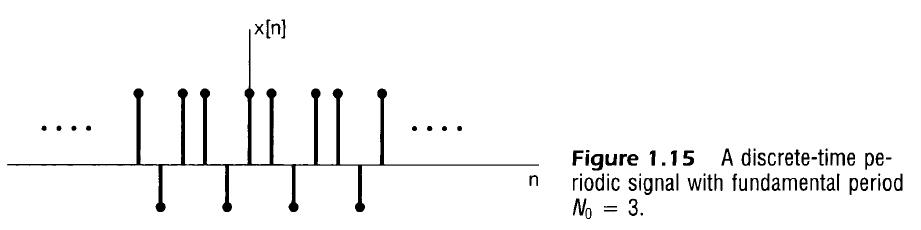
\includegraphics[width=\linewidth]{img/img27}
		\end{center}
	\end{itemize}
\end{frame}

\section{Sinyal Genap dan Ganjil}

\begin{frame}
	\frametitle{Sinyal genap dan ganjil}
	\begin{itemize}
		\item Sinyal genap
		$$ x(-t) = x(t) $$ atau $$ x[-n] = x[n] $$
		\item Sinyal ganjil
		$$ x(-t) = -x(t) $$ atau $$ x[-n] = -x[n] $$
	\end{itemize}
\end{frame}

\begin{frame}{Sinyal genap dan ganjil}
	\begin{center}
		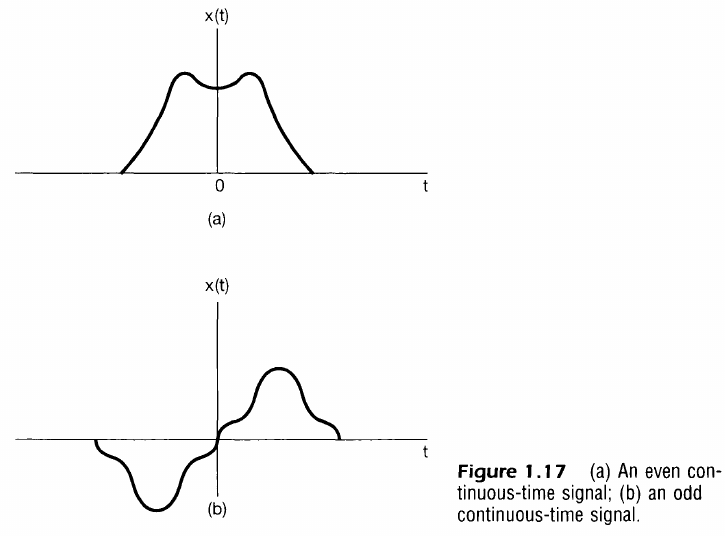
\includegraphics[width=0.8\linewidth]{img/img28}
	\end{center}
\end{frame}

\begin{frame}{Sinyal genap dan ganjil}
	\begin{itemize}
		\item Setiap sinyal dapat kita pecah menjadi penjumlahan dari dua sinyal
		\item Salah satunya adalah sinyal genap dan lainnya adalah sinyal ganjil.
		\begin{center}
			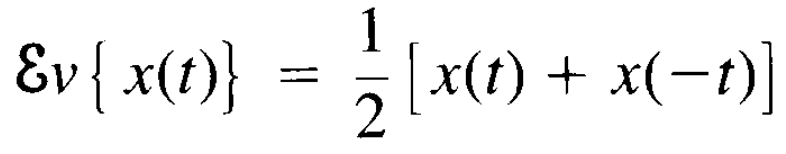
\includegraphics[width=0.5\linewidth]{img/img31}
		\end{center}
		\begin{center}
			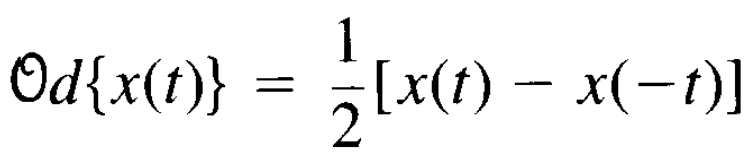
\includegraphics[width=0.5\linewidth]{img/img32}
		\end{center}
	\end{itemize}
\end{frame}

\begin{frame}{Sinyal genap dan ganjil}
	\begin{center}
		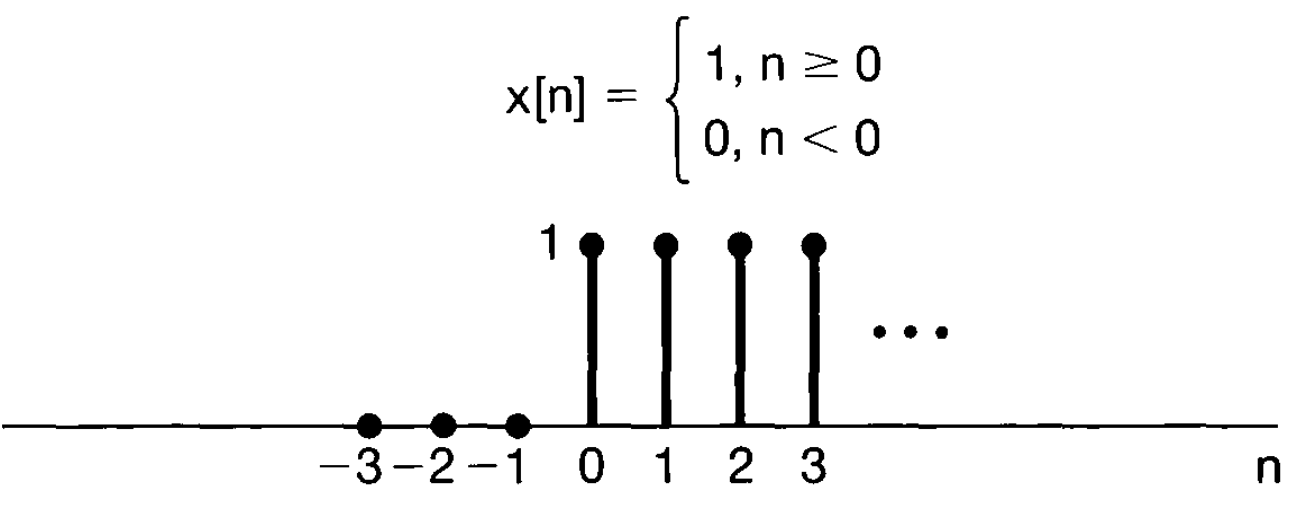
\includegraphics[width=0.8\linewidth]{img/img29}
	\end{center}
\end{frame}

\begin{frame}{Sinyal genap dan ganjil}
	\begin{center}
		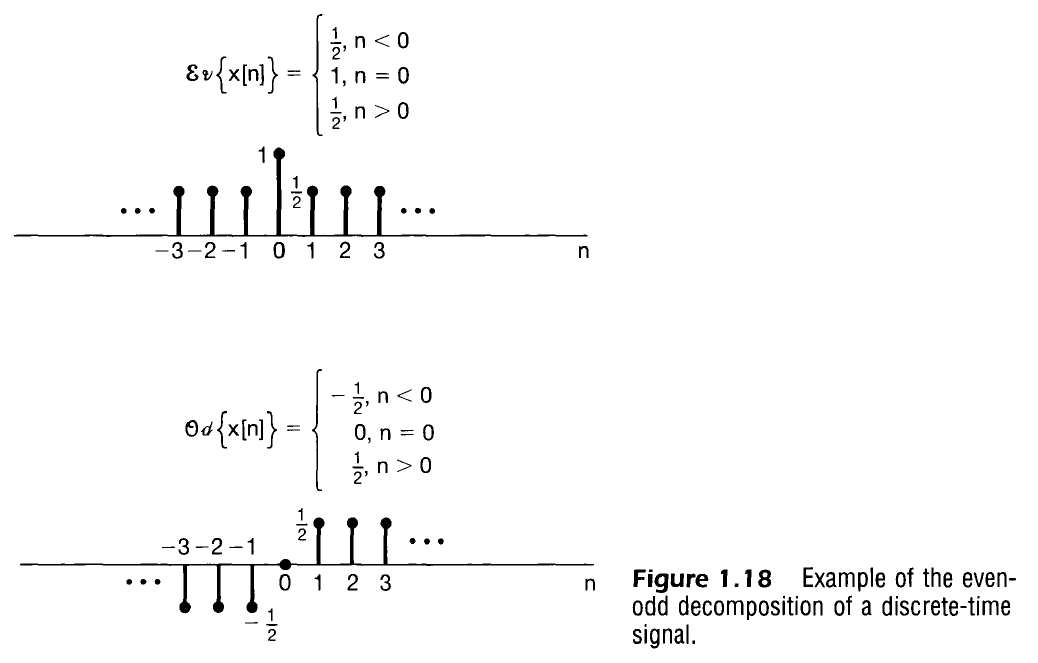
\includegraphics[height=0.8\textheight]{img/img30}
	\end{center}
\end{frame}

\section{Sinyal Eksponensial dan Sinusoidal}

\begin{frame}
	\frametitle{Sinyal eksponensial kompleks dan sinusoidal waktu kontinyu}
	\begin{itemize}
		\item Sinyal eksponensial kompleks waktu kontinyu
		$$ x(t) = Ce^{at} $$ dimana $ C $ dan $ a $ adalah bilangan kompleks.
		\item Berdasarkan parameter tersebut, eksponensial kompleks memiliki beberapa karakteristik yang berbeda.
	\end{itemize}
\end{frame}

\begin{frame}
	\frametitle{Sinyal eksponensial real}
	\begin{center}
		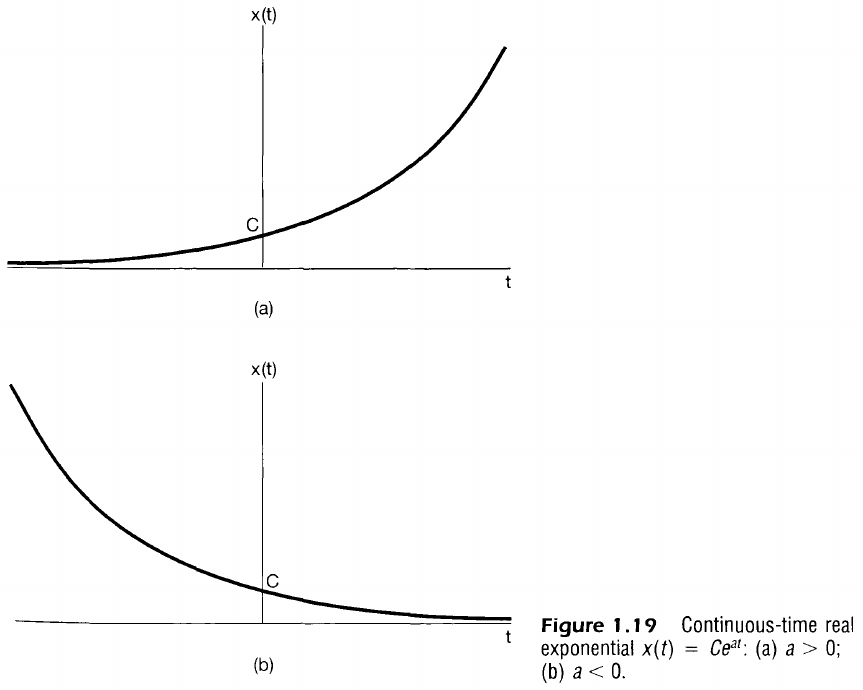
\includegraphics[width=0.7\linewidth]{img/img33}
	\end{center}
\end{frame}

\begin{frame}
	\frametitle{Sinyal eksponensial kompleks dan sinusoidal periodik}
	\begin{itemize}
		\item Jika $ a $: imajiner, maka
		$$ x(t) = e^{j\omega_0 t} $$ adalah sinyal periodik
		\item Pembuktian:\\
		syarat sinyal periodik
		\begin{align*}
			e^{j\omega_0 t} &= e^{j\omega_0 (t+T)} \\
			&= e^{j\omega_0 t} e^{j\omega_0 T}
		\end{align*}
		agar periodik maka $ e^{j\omega_0 T} = 1 $
	\end{itemize}
\end{frame}

\begin{frame}{Sinyal eksponensial kompleks dan sinusoidal periodik}
	\begin{itemize}
		\item Jika $ a $: imajiner, maka
		$$ x(t) = e^{j\omega_0 t} $$ adalah sinyal periodik
		\item Pembuktian:\\
		syarat sinyal periodik
		\begin{align*}
		e^{j\omega_0 t} &= e^{j\omega_0 (t+T)} \\
		&= e^{j\omega_0 t} e^{j\omega_0 T}
		\end{align*}
		agar periodik maka $ e^{j\omega_0 T} = 1 $
	\end{itemize}
\end{frame}

\end{document}
